\documentclass[a4paper, 12pt, final, garamond]{book}
\usepackage{cours-preambule}

\makeatletter
\renewcommand{\@chapapp}{Devoir maison 4 -- À rendre le 13 mai 2024}
\makeatother
\renewcommand{\thechapter}{}

\hfuzz=5.003pt

% \toggletrue{student}
% \toggletrue{corrige}
% \renewcommand{\mycol}{black}
% \renewcommand{\mycol}{gray}

\begin{document}
\setcounter{chapter}{3}

\settype{enon}
\settype{solu_prof}
\settype{solu_stud}

\chapter{\cswitch{Correction du DM}{DM~: Pompage optimal}}

\enonce{%
	On s'intéresse au gonflage d'un pneu de vélo à l'aide d'une pompe manuelle.
	On étudiera uniquement le premier coup de pompe, décrit ci-contre, pendant
	lequel la soupape $b$ reste toujours ouverte.
	\smallbreak
	\noindent
	\begin{minipage}[c]{.60\linewidth}
		Le volume de la pompe est $V_p = \SI{2.0}{L}$, celui de la chambre à air
		est $V_0 = \SI{5.0}{L}$ (constant), et l'ensemble est initialement à la
		pression $P_0 = \SI{1}{bar}$ et à la température $T_0 = \SI{300}{K}$. On
		note 1 l'état initial et 2 l'état final. On envisage deux moyens de réaliser
		la compression 1 $\to$ 2~:
		\begin{itemize}
			\item[b]{Compression lente}~: dans ce cas les échanges thermiques ont le
			temps de s'établir, et la température reste constante et égale à $T_0$~;
			\item[b]{Compression brusque}~: dans ce cas la température du gaz va
			augmenter et il faudra, après la compression, attendre qu'elle redescende
			à $T_0$.
		\end{itemize}
		On suppose dans les deux cas la transformation mécaniquement réversible, et le
		gaz est modélisé par un gaz parfait d'indice adiabatique $\gamma = \num{1.4}$.
	\end{minipage}
	\hspace*{\fill}
	\begin{minipage}[c]{.30\linewidth}
		\begin{center}
			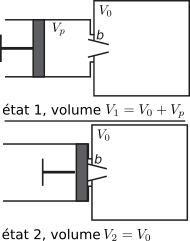
\includegraphics[width=\linewidth]{pompage-plain}
		\end{center}
	\end{minipage}
}%
\QR{%
	Dans le premier cas, que valent la température et le volume final~? Donner
	ensuite l'expression de la pression finale $P_2$ en fonction de $P_0$ et
	$\alpha = V_p/V_0$. La calculer.
}{%
	La transformation est la suivante~:
	\[
		\text{État initial~}
		\left|
		\begin{array}{l}
			P_1 = P_0 = \SI{1}{bar}
			\\
			V_1 = V_0 + V_p
			\\
			T_1 = T_0
			\\
			n_1
		\end{array}
		\right.
		\quad
		\opto{\text{isotherme}}{\text{G.P.}}
		\quad
		\text{État final~}
		\left|
		\begin{array}{l}
			P_2 = ~?
			\\
			V_2 = V_0
			\\
			T_2 = T_0
			\\
			n_2 = n_1
		\end{array}
		\right.
	\]
	$T$ et $n$ étant constants, on a $P_0V_1 = nRT_0 = P_2V_2$, soit
	\begin{gather*}
		P_0 (V_0+V_p) = P_2V_0
		\Lra
		\boxed{P_2 = P_0 (1+\alpha)}
		\qav
		\left\{
		\begin{array}{rcl}
			P_0 & = & \SI{1}{bar}
			\\
			V_p & = & \SI{2.0}{L}
			\\
			V_0 & = & \SI{5.0}{L}
		\end{array}
		\right.\\
		\AN
		\xul{
			P_2 = \SI{1.4}{bar}
		}
	\end{gather*}
}%
\QR{%
	Justifier que ces valeurs sont les mêmes dans le second cas.
}{%
	Le volume final est évidemment le même~: $V_2 = V_0$. La température l'est
	aussi, puisqu'on attend suffisamment longtemps pour que ça soit le cas~: $T_2
		= T_0$. On a également $n_2 = n_1$. La pression finale est donc
	\[
		P_2 = \frac{n_2RT_2}{V_2} = \frac{n_1RT_0}{V_0} = \frac{P_0(V_0+V_p)}{V_0} =
		P_0 (1+\alpha)
	\]
	donc identique au cas précédent.
}%
\QR{%
	Dans le premier cas, donner l'expression du travail à fournir au gaz pour le
	comprimer en fonction de $P_0$, $V_1$ et $\alpha = V_p/V_0$. Faire
	l'application numérique.
}{%
	C'est une compression isotherme $(T = T_0 = \cte)$ et mécaniquement réversible
	$(P = P\ind{ext})$ d'un gaz parfait $(P = nRT_0/V)$~:
	\begin{gather*}
		W_{12} =
		-\int_{V_1}^{V_2} P\ind{ext}\dd{V} =
		-n_1RT_0\int_{V_1}^{V_2} \frac{\dd{V}}{V} =
		-n_1RT_0 \ln \frac{V_2}{V_1}
		\intertext{Or $n_1RT_0 = P_0V_1$, $V_1 = V_0+V_p$ et $V_2 = V_0$, soit}
		\boxed{W_{12} = P_0V_1 \ln (1+\alpha)}
		\Ra
		\xul{W_{12} = \SI{236}{J}}
	\end{gather*}
}%
\begin{blocQR}
	\item
	\enonce{%
		Dans le second cas, il faut décomposer la transformation en deux étapes~: de
		l'état 1 à un état 1'. Il s'agit de la compression où le volume passe de
		$V_1 = V_0+V_p$ à $V_{1'} = V_0$, puis de l'état 1' à l'état 2 le volume ne
		change plus et le gaz se refroidit jusqu'à $T_0$.
	}%
	\QR{%
		Expliquer pourquoi l'étape $1 \to 1'$ peut être supposée adiabatique et
		mécaniquement réversible.
	}{%
		L'étape $1\to 1'$ est réalisée rapidement, donc les transferts thermiques
		n'ont pas le temps de s'établir~: on peut la supposer adiabatique. De plus,
		l'énoncé indique qu'elle est supposée réversible, c'est-à-dire qu'on néglige
		tout frottement.
	}%
	\QR{%
		Calculer la température atteinte en 1' grâce à une des loi de
		\textsc{Laplace}.
		% TODO: Ajouter variables à utiliser
	}{%
		On est en présence d'un gaz parfait lors d'une transformation adiabatique et
		mécaniquement réversible entre les états 1 et 1', on peut donc utiliser la
		loi de \textsc{Laplace}~:
		\begin{gather*}
			T_1V_1^{\gamma-1} = T_{1'}V_{1'}^{\gamma-1}
			\qso
			T_{1'} = T_1 \left( \frac{V_1}{V_{1'}} \right)^{\gamma-1}
			\intertext{Or $T_1 = T_0$, $V_1 = V_0+V_p$ et $V_{1'} = V_0$, donc}
			\boxed{T_{1'} = T_0 (1+\alpha)^{\gamma-1}}
			\Ra
			\xul{T_{1'} = \SI{343}{K}}
		\end{gather*}
	}%
	\QR{%
		Calculer le travail à fournir au gaz durant l'évolution $1 \to 1' \to 2$.
		% TODO: Ajouter variables à utiliser (littéral avant)
	}{%
		On décompose la transformation en deux étapes~:
		\begin{itemize}
			\item De 1 à 1', on a une transformation adiabatique mécaniquement
			      réversible d'un gaz parfait. On peut soit calculer le travail
			      directement, soit utiliser le premier principe~:
			      \begin{itemize}
				      \item[b]{Premier principe}
				      \begin{DispWithArrows*}[]
					      \Delta{U} &= C_V\Delta{T}
					      \\\Lra
					      W + Q &= \frac{nR}{\gamma-1} (T_{1'} - T_1)
					      \Arrow{$Q = 0$\\Factorisation par $T_1$}
					      \\\Lra
					      W &= \frac{nRT_1}{\gamma-1} \left( \frac{T_{1'}}{T_1} - 1 \right)
					      \Arrow{Adiabatique réversible G.P.\\$T_1V_1^{\gamma-1} =
					      T_{1'}V_{1'}^{\gamma-1}$}
					      \\\Lra
					      \Aboxed{
						      W &= \frac{P_1V_1}{\gamma-1}
						      \left(\left( \frac{V_{1'}}{V_1} \right)^{1-\gamma} - 1\right)
					      }
				      \end{DispWithArrows*}
				      \item[b]{Calcul direct}
				      \begin{DispWithArrows*}
					      W &= -\int_{V_1}^{V_{1'}} P\ind{ext}\dd{V}
					      \Arrow{Mécaniquement réversible\\$P\ind{ext} = P$}
					      \\\Lra
					      W &= -\int_{V_1}^{V_{1'}} P\dd{V}
					      \Arrow{Adiabatique réversible G.P.\\$P = P_1 \frac{V_1^{\gamma}}{V^{\gamma}}$}
						      \\\Lra
						      W &= -P_1V_1^{\gamma} \int_{V_1}^{V_{1'}} \frac{\dd{V}}{V^{\gamma}}
						      \Arrow{$\DS\int x^n \dd{x} = \frac{x^{n+1}}{n+1}$}
						      \\\Lra
						      W &=
						      -P_1V_1^{\gamma}
						      \left[\frac{V^{-\gamma+1}}{-\gamma+1}\right]_{V_1}^{V_{1'}}
						      \Arrow{On calcule}
						      \\\Lra
						      W &= -\frac{P_1V_1^{\gamma}}{-\gamma+1} (V_{1'}^{1-\gamma} -
						      V_1^{1-\gamma})
						      \Arrow{On factorise par $V_1^{1-\gamma}$}
					      \\\Lra
					      W &=
					      -\frac{P_1V_1^{\cancel{\gamma}}}{-\gamma+1}
					      V^{1-\cancel{\gamma}}
					      \left(\left( \frac{V_{1'}}{V_1} \right)^{1-\gamma} - 1\right)
					      \Arrow{On simplifie les $-$}
					      \\\Lra
					      \Aboxed{
						      W &= \frac{P_1V_1}{\gamma-1}
						      \left(\left( \frac{V_{1'}}{V_1} \right)^{1-\gamma} - 1\right)
					      }
				      \end{DispWithArrows*}
			      \end{itemize}
			      Dans tous les cas, avec $P_1 = P_0$, $V_{1'} = V_0$ et $V_1 = V_0+V_p$,
			      on obtient
			      \[
				      \xul{W = \SI{252}{J}}
			      \]
			\item De 1' à 2, on a une transformation isochore, de travail nul.
		\end{itemize}
	}%
\end{blocQR}
\QR{%
	Tracer sur un même diagramme $(P,V)$ les deux transformations. Pouvait-on
	prédire le fait que le travail à fournir est plus grand pour une des deux
	compressions~? À quoi a servi le surplus de travail fourni dans celle qui en
	nécessite le plus~? Conclure sur la meilleure méthode.
}{%
	\noindent
	\begin{minipage}[t]{.4\linewidth}
		Dans un diagramme $(P,V)$, le travail des forces de pression reçu par le gaz
		est égal à l'aire sous la courbe. Or, la compression \textbf{adiabatique
			mécaniquement réversible} dessine une \textbf{aire plus importante}~: on
		pouvait donc \textbf{prédire que $W\ind{brusque} > W\ind{lente}$}.
		\bigbreak
		Ce travail a servi a \textbf{chauffer le gaz}, jusqu'à \SI{343}{K}. Ceci
		n'est cependant \textbf{pas utile} puisque le gaz refroidit ensuite.
		Cette énergie thermique est dissipée vers la pièce et \textbf{n'est pas
			récupérable}.
	\end{minipage}
	\hfill
	\begin{minipage}[t]{.55\linewidth}
		\begin{center}
			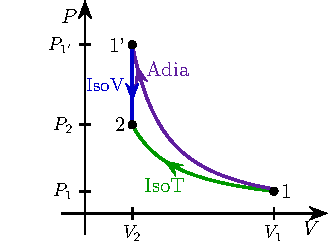
\includegraphics[width=\linewidth]{adia_vs_isoT}
		\end{center}
	\end{minipage}
	Ainsi, tout est une question de temps~: si on n'est pas pressé, il vaut mieux
	\textbf{pomper lentement}~!
}%

\enonce{%
	\begin{tcn}(rema){Utilité en industrie}
		Ce qui précède a des conséquences pratiques importantes à l'échelle
		industrielle. Il existe en effet des stations qui stockent de l'air comprimé
		dans d'immenses réservoirs (souvent des cavités géologiques) et qui
		réutilisent ensuite cet air pour faire tourner une turbine et produire de
		l'électricité. La phase de compression de l'air doit consommer le moins
		possible d'énergie, et ce qui précède montre donc qu'elle a intérêt à être
		proche de l'isotherme réversible. Cf.\ par exemple \url{https://www.connaissancedesenergies.org/fiche-pedagogique/caes-stockage-par-air-comprime}.
	\end{tcn}
}%

\end{document}
